\chapter{Critical period plasticity in fragile X mice}

\section{Overview}
\newrefsection

Fragile X syndrome (FXS), the most common form of heritable mental retardation, is a developmental disorder with known effects within sensory systems. Altered developmental plasticity has been reported in the visual and somatosensory systems in \textit{Fmr1} knock-out (KO) mice. Behavioral studies have revealed maladaptive auditory responses in FXS patients and \textit{Fmr1} KO mice, suggesting that adaptive plasticity may also be impaired in the auditory system. Here we show that, whereas tonotopic frequency representation develops normally in \textit{Fmr1} KO mice, developmental plasticity in primary auditory cortex is grossly impaired. This deficit can be rescued by pharmacological blockade of mGluR5 receptors. These results support the mGluR hypothesis of fragile X mental retardation and suggest that deficient developmental plasticity may contribute to maladaptive auditory processing in fragile X syndrome.

\section{Introduction}

Fragile X syndrome (FXS) is caused by expansion of trinucleotide CGG repeats in the \textit{Fmr1} gene resulting in hypermethylation and loss of function of the gene (\cite{Jin2003}). \textit{Fmr1} encodes fragile X mental retardation protein (FMRP), an mRNA-binding protein that suppresses and regulates local mRNA translation. The lack of FMRP exaggerates mGluR-stimulated protein synthesis, which has been hypothesized to cause various fragile X symptoms (\cite{Bear2004, Osterweil2010}). Supporting this mGluR hypothesis of fragile X syndrome, the blockade of mGluR either genetically or pharmacologically reverses certain fragile X phenotypes in animal models (\cite{McBride2005, Yan2005, Dolen2007, DeVrij2008, Meredith2011, Su2011, Michalon2012, Thomas2012}).

Fragile X mental retardation is the most common form of heritable mental retardation. Among its symptoms are maladaptive sensory responses and impaired sensory integration (\cite{Miller1999, Chen2001, Nielsen2002}), which have been hypothesized to contribute to the impaired development of higher cognitive functions (\cite{Hanson, Leblanc2011}). Studies in mouse models lacking the \textit{Fmr1} gene revealed altered ocular dominance plasticity in visual cortex and a delayed critical period of synaptic plasticity in barrel cortex (\cite{Dolen2007, Harlow2010a}). Altered auditory processing in humans with fragile X syndrome and \textit{Fmr1} knock-out (KO) animals suggests that development and plasticity in the auditory system may also be affected by fragile X syndrome (\cite{Miller1999, Chen2001, Nielsen2002}).

The development of acoustic representations in primary auditory cortex is profoundly influenced by early experience (\cite{Zhang2001, DeVillers-Sidani2007, Insanally2009, Popescu2010a}). Exposure of juvenile animals to patterned sensory input refines the balance of excitation and inhibition (\cite{Dorrn2010, Sun2010}), resulting in receptive field and sensory map reorganization and a long-lasting impact on sound perception (\cite{Han2007}). The robust effects of early experience on sound representation and perception make the auditory cortex an ideal system to investigate how genetic mutations may lead to sensory abnormalities, such as those caused by fragile X mental retardation and \textit{Fmr1} gene deletion. In addition, cellular and synaptic abnormalities have been well characterized in the \textit{Fmr1} KO mouse, making it a valuable model to study the mechanisms of sensory development and plasticity.

In the present study, we investigate the development of cortical sound representations and sound-induced cortical map reorganization in the \textit{Fmr1} KO mouse. Our results indicate that the \textit{Fmr1} KO mouse develops a normal tonotopic cortical frequency map, but does not show experience-dependent map reorganization. Systemic administration of MPEP, an mGluR5 antagonist, rescues the impairment in cortical map plasticity.

\section{Methods}

\subsection{Rearing and injection procedures}

All procedures used in this study were approved by the Animal Care and Use Committee at the University of California, Berkeley. Wild-type (WT) and \textit{Fmr1} KO mice on the FVB background were originally obtained from The Jackson Laboratory (FVB.129P2-Pde6b\textsuperscript{+} Tyr\textsuperscript{c-ch}/AntJ and FVB.129P2-Pde6b\textsuperscript{+} Tyr\textsuperscript{c-ch} Fmr1\textsuperscript{tm1Cgr}/J). Only male homozygous WT or KO mice were used in this study. Litters of mouse pups were placed in sound-attenuating chambers with their mothers from postnatal day 9 (P9) through P20 (early window) and exposed to 16 kHz pure tone pips (25 ms duration, 60 dB SPL) presented in trains of 6 pips (each train every 2 s and pips presented at 5 pips per second within a train) through an overhead speaker. Additional juvenile mice were exposed to the same sound stimuli at a later time window (P20-P30). Animals reared in a normal laboratory husbandry setting served as na\"ive controls.

Additional litters of animals, exposed to the same sound stimuli during either the early (P9-P20) or the late window (P20-P30), were also given daily injections of 2-methyl-6-(phenylethynyl)-pyrydine (MPEP; reconstituted to 2 mg/ml, injected at 30 mg/kg, i.p.; Sigma-Aldrich) or vehicle saline (15 ml/kg, i.p.). The weights of these animals were monitored daily to ensure proper development. Consistent with previous reports (\cite{Moy2009}), KO animals generally had larger body mass than WT animals. Sound exposure tended to reduce weight gain of KO animals and increase weight gain of WT animals (Table 1).

\begin{figure}
	\centering
		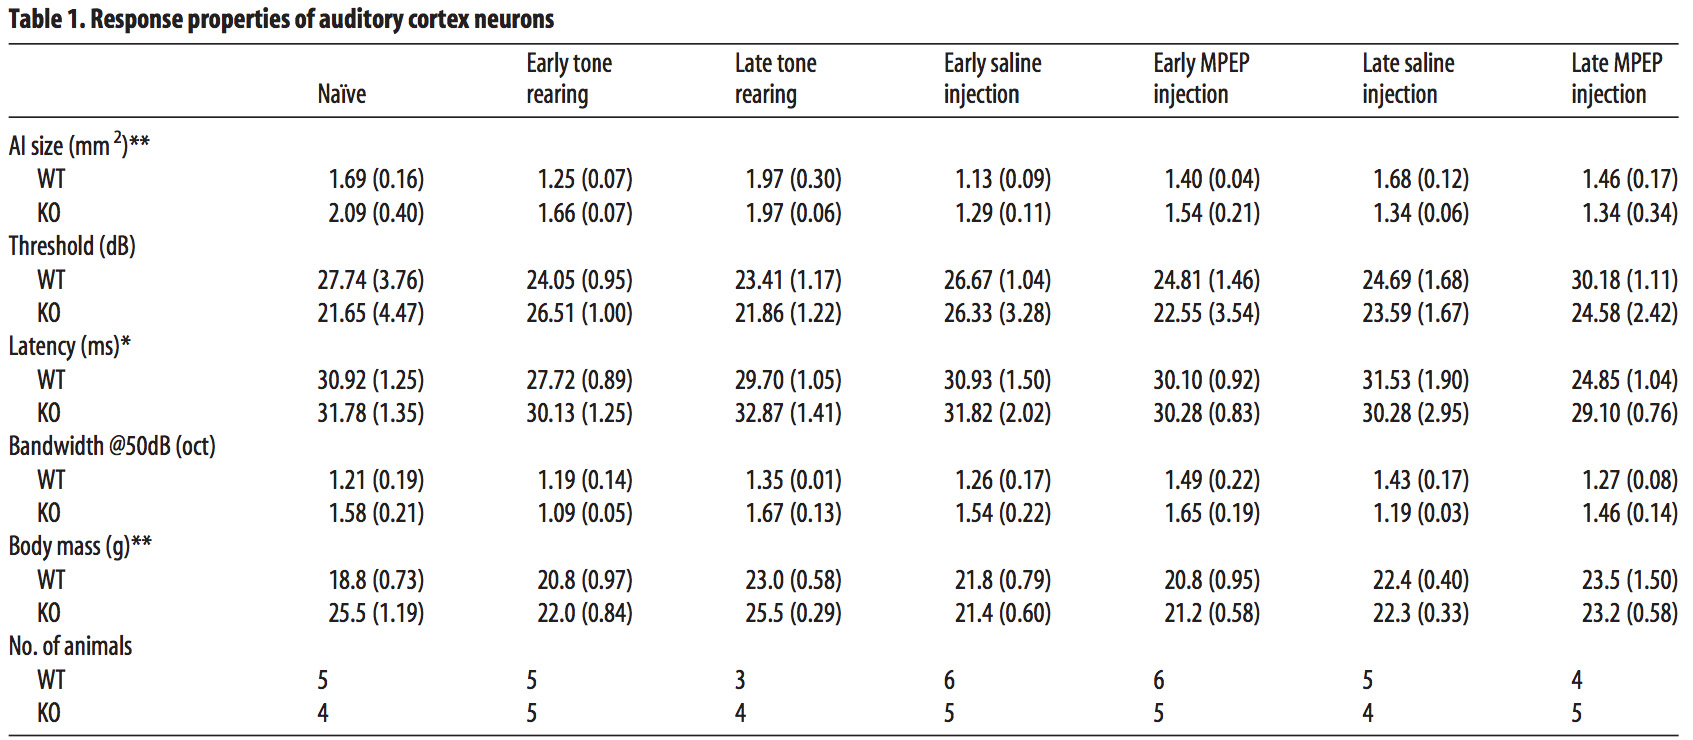
\includegraphics[width=7in]{images/C2T1}
	\begin{changemargin}{1in}{1in}
	\footnotesize{Table 1. AI size, threshold, peak latency, bandwidth at 50 dB, body mass, and number of animals used in all conditions. SEM is shown in parentheses. Two$\times$7 ANOVAs (genotype $\times$ condition) showed significant effects for overall size, latency, and body mass. Significant main effects for condition were found for overall size of AI (**$p<0.005$) and latency (*$p<0.05$), but not for genotype or interaction. Significant main effects for genotype ($p<0.005$) and condition ($p<0.005$), and a significant interaction ($p<0.001$) were found for body mass.}
	\end{changemargin}
\end{figure}

After sound exposure, experimental animals were returned to a normal laboratory husbandry setting until the electrophysiological mapping of primary auditory cortex (typically P35-P45). A subset of early window exposure animals were recorded immediately after removal from the sound exposure box (P20-P25). Care was taken to ensure that all conditions (genotype, exposure, injection schedule) were age-matched during mapping, except the subset of animals that were mapped immediately after removal from the sound exposure box. Across the 16 conditions, a total of 76 animals were used for cortical electrophysiological experiments (Table 1). An additional 16 animals were used for auditory brainstem responses (ABRs).

\subsection{Electrophysiological recording procedure}

The primary auditory cortex (AI) of mice was mapped as previously described (\cite{Kim2009}), except as follows. Mice were anesthetized with ketamine (100 mg/kg, i.p.) and xylazine (10 mg/kg, i.p.), and supplemented as needed (ketamine 50 mg/kg, xylazine 5 mg/kg, i.p. generally once an hour). The cortex was maintained under a layer of silicone oil, reapplied as necessary. Multiunit responses to 25 ms pure tone pips (2-74 or 4-74 kHz, 0.1 octave increments at 0-70 dB SPL, 10 dB increments) were recorded using tungsten microelectrodes (FHC) in the thalamorecipient layer of AI (350-450 \textmu{}m below the cortical surface). References to neurons in this text refer to multiunit responses recorded extracellularly. Tones were presented to the left ear through an electrostatic speaker (Tucker Davis Technologies) at 3 pips per second and each frequency-intensity combination was repeated three times. Cortical penetration locations were recorded on a magnified high-resolution image.

ABRs were recorded under identical anesthetic conditions with the active electrode at the vertex, the reference electrode caudomedial to the left ear pinna, and the ground electrode at the dorsosacrum (\cite{OConnor1998, Popescu2010}). Tone pips (4, 8, 16, and 32 kHz at 0-70 dB SPL in 5 dB increments) were presented to the left ear and ABRs were recorded ipsilaterally. Responses to 500 pips were averaged and high-pass filtered with a cutoff frequency of 200 Hz.

\subsection{Data analysis}

Receptive fields and response properties were isolated using custom-made programs in MATLAB as previously described (\cite{Insanally2010}), except as follows. The peak of the peristimulus time histogram (PSTH) within a window from 7 to 50 ms after the stimulus onset was defined as the response latency. The response window was defined as a period encompassing the PSTH peak, in which the firing rate was higher than the baseline firing rate. The spikes in the response window were counted to reconstruct the receptive field. The characteristic frequency (CF) and threshold of the receptive fields were identified by hand by a blind experimenter. Bandwidth at 50 dB SPL was automatically calculated as previously described (\cite{Insanally2010}).

ABR thresholds at each frequency were determined as the lowest intensity that produced a visibly discernible response. Wave latency times were manually labeled for two frequency (8 and 16 kHz) and two intensity levels (70 and 45 dB SPL). Wave amplitudes were calculated as the amplitude from a peak to an ensuing trough.

All error bars indicate SEM. N-way ANOVAs are employed throughout using the following conditions and groups: Genotype (wildtype and knockout), Exposure (na\"ive and exposed), and Frequency (0.4 octave bins). Statistical tests are indicated in the text.

\section{Results}

\subsection{\textit{Fmr1} KO mice exhibit impaired critical period sensory map plasticity}

Litters of WT and KO animals were exposed to 16 kHz tones from P9 to P20. This window encompasses the critical period for frequency representation in rats (\cite{DeVillers-Sidani2007, Insanally2009}) and has been shown to elicit map plasticity in mice (\cite{Barkat2011}). Na\"ive WT and KO animals had very similar cortical frequency representation (Fig. 1A,B), suggesting normal auditory cortex development in KO mice. WT animals exposed to 16 kHz tone showed a substantial increase in representation of 16 kHz, whereas KO animals exposed to the same tone did not (Fig. 1A,B). A 2$\times$2$\times$10 ANOVA (genotype $\times$ exposure $\times$ frequency bin) revealed a significant three-way interaction ($p=0.0009$), suggesting a differential representation to specific frequency bins between genotype and rearing condition. A further two-way ANOVA (genotype $\times$ exposure) on individual frequency bins found significant effects at 16 kHz (exposure condition, $p=0.00029$; genotype, $p=0.055$; interaction $p=0.024$; Fig. 1B), indicating representation of the exposed frequency increased in the WT mice only. The sound exposure had opposite effects on the representation of 21.11 kHz for the two genotypes (two-way ANOVA interaction, $p=0.0002$), reducing 21.11 kHz representation in the WT but not KO mice. Similar reduction of representations for frequencies near the exposure frequency has been previously reported (\cite{Han2007}).

This impairment in plasticity could be due to a delay in the critical period (\cite{Harlow2010a}). To address this possibility, additional litters of animals were exposed to 16 kHz between P20 and P30. A 2$\times$3 ANOVA (genotype $\times$ exposure) revealed a significant main effect for exposure condition ($p=0.0001$) and a significant interaction ($p=0.015$). We find that only the WT mice that were sound exposed in the early window, but not the late window, had enlarged representation of 16 kHz (Fig. 1C). Neither the WT nor the KO mice that were sound-exposed in the late window showed enhanced representations of 16 kHz. Thus, the critical period for frequency-representation in mice does not extend beyond P20, and KO mice do not have a delayed critical period.

\begin{figure}[p]
	\centering
		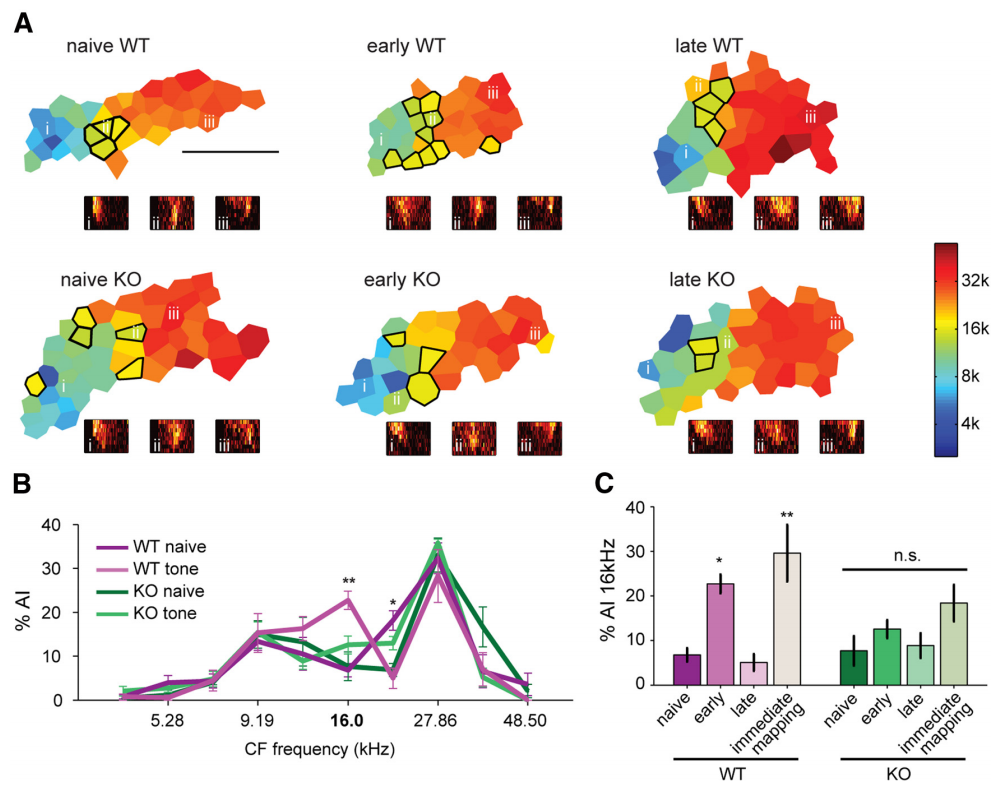
\includegraphics[width=6in]{images/C2F1}
	\begin{changemargin}{1in}{1in}
	\footnotesize{Figure 1. \textit{Fmr1} KO mice exhibit impaired critical period plasticity in the auditory cortex. (A) Example AI frequency maps of two genotypes (WT and \textit{Fmr1} KO) and three conditions (na\"ive, early tone exposure, late tone exposure). Areas outlined in black indicate sites with CFs near the exposure frequency of 16 kHz ($\pm0.2$ octaves). Example receptive fields are shown for each map, with the location indicated by white roman numerals (x-axis is frequency from 2-74 kHz; y-axis is sound level from 0 to 70 dB). Scale bar, 1 mm. (B) Size of frequency representation for the na\"ive and early tone exposure groups. The WT early tone exposure group shows a significant increase in representation of 16 kHz (**condition main effect $p=0.00029$ and interaction $p=0.024$). A small decrease is also observed at 21.1 kHz (*interaction $p=0.0002$). (C) Representation of 16 kHz across four conditions (same as (A) with the addition of early tone exposure animals mapped immediately after removal from tone exposure box). Early tone exposure resulted in a significant increase in 16 kHz representation in the WT animals in both mapping windows (one-way ANOVA main effect $p<0.0005$, post hoc tests: *$p<0.05$ and **$p<0.005$). Sound exposure did not cause map changes in KO animals (one-way ANOVA, $p=0.13$).}
	\end{changemargin}
\end{figure}


The lack of exposure-induced frequency map reorganization in the KO mice could also be due to previously reported hyperplasticity (\cite{Dolen2007}), which might have allowed a rapid reversal of the altered frequency map during the period of normal sensory experience before the auditory cortex was mapped. To address this possibility, additional litters of animals (WT: n = 4; KO: n = 6) were exposed to 16 kHz continually from P9 until the day of AI mapping (P20-P25; Fig. 1C). A one-way ANOVA comparing 16 kHz representation in na\"ive, early exposure, and early exposure immediately mapped WT animals reveal a significant effect ($p=0.0022$), with post hoc analyses showing no significant differences between the two early exposure groups that were mapped at different ages. A similar ANOVA on the KO animals shows a nonsignificant effect ($p=0.135$). Although the immediately mapped KO animals appear to show a slight increase in representation of 16 kHz, even an uncorrected comparison of the KO na\"ive and immediately mapped animals did not show a significant effect ($p=0.0988$).

\subsection{Auditory brainstem response differences are not frequency specific}

\textit{Fmr1} KO animals are impaired in experience-dependent regulation of potassium channels in the auditory brainstem (\cite{Strumbos2010}). To investigate potential subcortical plasticity, we compared ABRs between WT and KO mice that were either na\"ive or 16 kHz-exposed (P9-P20; Fig. 2A). Sound exposure reduced the ABR amplitude in WT mice and increased the amplitude in KO mice (genotype $\times$ exposure $\times$ frequency $\times$ intensity repeated measures four-way ANOVA: genotype effect, $p=0.038$; exposure, $p=0.0069$; their interaction, $p<0.0001$; Fig. 2B). However, this effect does not appear to be frequency specific, as the frequency interactions with genotype ($p=0.53$) and exposure ($p=0.41$) are not significant. The ABR threshold was not different between the genotypes and was not altered by sound exposure (ANCOVA on genotype $\times$ exposure with frequency as a covariate: genotype, $p=0.587$; exposure, $p=0.909$; interaction, $p=0.0609$; Fig. 2C).

\begin{SCfigure}
  \centering
  	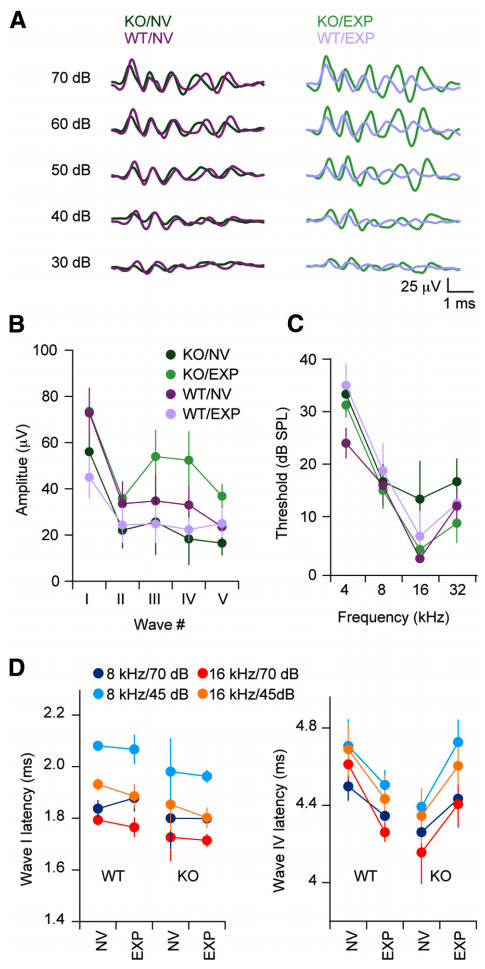
\includegraphics[width=0.6\textwidth]{images/C2F2}
  \captionsetup{labelformat=empty}
  \caption{\footnotesize{Figure 2. ABRs are altered in \textit{Fmr1} KO mice, but not in a frequency-specific manner. (A) Example ABR traces recorded from WT and KO animals that were either na\"ive (NV, left) or 16 kHz-exposed (EXP, right). Responses were activated by 16 kHz tone pips. (B) Amplitudes of the five ABR waves recorded with 16 kHz tone pips at 70 dB. Sound exposure had different effects on WT and KO mice, increasing ABR amplitudes in KOs and reducing ABR amplitudes in WTs (genotype $\times$ exposure interaction, $p<0.0001$). (C) The ABR threshold was not different between the genotypes and was not altered by sound exposure. (D) Latencies of wave I (left) and wave IV (right). Latency for wave I was shorter for KOs than WTs ($p=0.0073$) and was not altered by sound exposure. Latency for wave IV was shortened by sound exposure in WTs, but delayed in KOs (genotype $\times$ exposure interaction, $p<0.001$). These effects were consistent across frequency (8 and 16 kHz) and sound level (45 and 70 dB).}}
\end{SCfigure}

ABR latency was analyzed with two-way ANOVAs (genotype $\times$ exposure) for each discernible wave. In wave I, which represents early responses in the auditory nerve, KO mice had shorter latencies than WT mice and this difference was not altered by experience (genotype, $p=0.0073$; sound exposure, $p=0.87$; interaction, $p=0.55$; Fig. 2D). No significant effects were found for wave II or wave III, which represent responses from the spiral ganglion and cochlear nucleus, respectively (data not shown). Sound exposure reduced latencies in the WT groups, but increased them in the KO groups for waves IV and V, which represent responses from the superior olivary complex and inferior colliculus, respectively (interaction, $p<0.001$ and $p=0.006$, respectively; Fig. 2D). These effects were consistently seen for both the exposed (16 kHz) and nonexposed (8 kHz) frequencies, and at 45 and 70 dB sound pressure levels (Fig. 2D). These results indicate that, although FMRP deficiency and sound exposure significantly impacted ABRs, the effects are frequency-nonspecific and therefore cannot account for frequency-specific map reorganization in AI. Furthermore, the ABRs in the KO mice are not grossly impaired, and the ABR differences probably do not account for the impairment in auditory map plasticity.

\subsection{Daily injection of MPEP rescues plasticity deficit in KO mice}

It has been suggested that fragile X phenotypes are related to overactive Group 1 metabotropic glutamate receptors (\cite{Bear2004}). Indeed, genetic manipulations to suppress mGluR5 have been shown to rescue many fragile X phenotypes (\cite{Dolen2007}). In addition, pharmacological suppression of mGluR5 using MPEP or CTEP has been shown to correct many deficits in both mouse and Drosophila melanogaster models of fragile X syndrome (\cite{McBride2005, Yan2005, DeVrij2008, Meredith2011, Su2011, Michalon2012, Thomas2012}).

To investigate the role of mGluR in auditory critical period plasticity, we exposed additional litters of mice to 16 kHz during either the early (P9-P20) or late (P20-P30) window and systemically administered either MPEP or vehicle saline to littermates daily. We found that both MPEP- and saline-injected WT animals had larger representations of 16 kHz than na\"ive WT animals when they were exposed in the early window, but not the late window (Fig. 3A). A one-way ANOVA on the WT animals across the five conditions revealed a significant effect ($p=0.023$), with the early window saline and MPEP groups having significantly larger 16 kHz representations than the na\"ive groups ($p<0.05$ and $p<0.005$, respectively; post hoc least significant difference (LSD); Fig. 3B). The two late window groups did not differ from the na\"ive group, suggesting that saline or MPEP injection does not enhance plasticity outside the normal critical period in WT animals ($p>0.05$). In the KO animals, only those exposed to 16 kHz between P9-P20 in conjunction with daily MPEP injection showed an increase in representation of 16 kHz (Fig. 3C). A one-way ANOVA on the KO animals across the five conditions revealed a significant effect ($p=0.0021$), driven exclusively by the early window MPEP group ($p<0.001$, compared with na\"ive, post hoc LSD). The four remaining groups show no significant differences ($p>0.05$, for all). Our data suggest that although the blockade of mGluR5 does not interfere with critical period map plasticity in WT animals, such a blockade is sufficient to rescue the plasticity deficit observed in KO animals within the classical critical period window.


\begin{figure}[p]
	\centering
		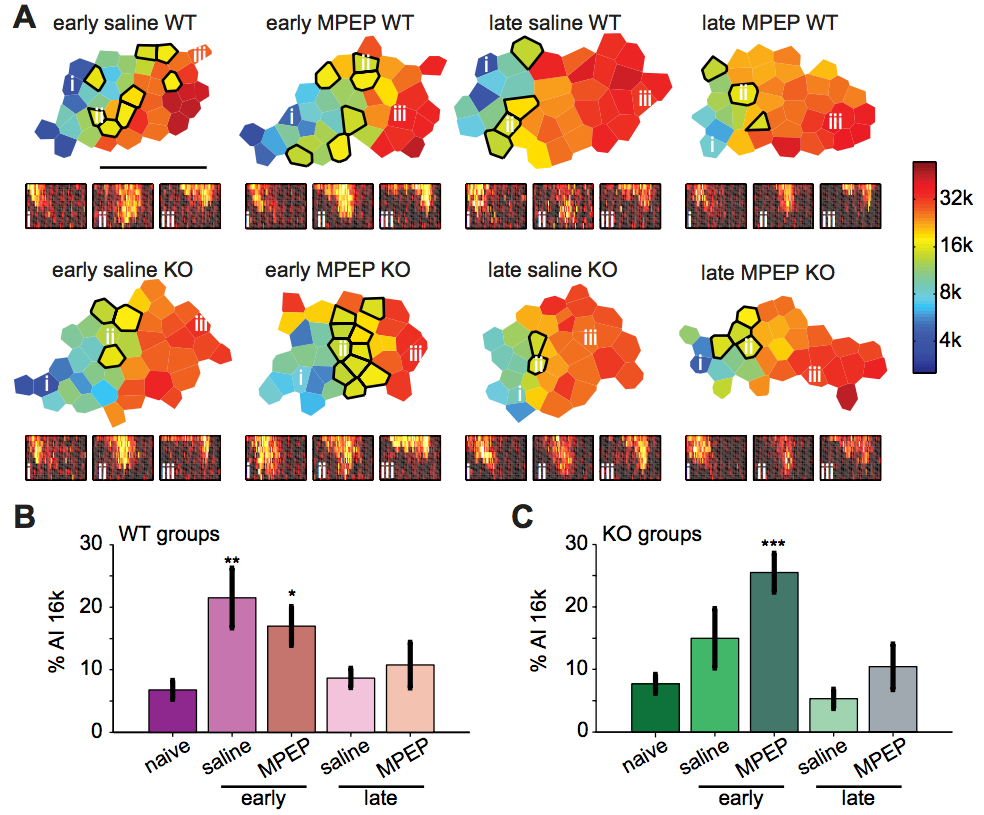
\includegraphics[width=6in]{images/C2F3}
	\begin{changemargin}{1in}{1in}
	\footnotesize{Figure 3. MPEP injections rescue plasticity deficit. (A) Example maps of WT and KO animals injected daily with either vehicle saline or MPEP while being exposed to 16 kHz during an early window (P9-P20) or a late window (P20-P30). Areas outlined in black indicate sites with CFs near the exposure frequency of 16 kHz ($\pm0.2$ octaves), as in Figure 1. Example receptive fields are shown for each map; location of receptive the field is indicated by white roman numerals (x-axis is frequency from 2 to 74 kHz; y-axis is dB from 0 to 70 dB). Scale bar indicates 1 mm. (B) Representation of 16 kHz in AI of WT animals. Naive group is the same as shown in Figure 1C. A significant increase in representation (compared with the naive group) was observed for both early window saline and MPEP injection groups. (C) Representation of 16 kHz in AI of KO animals. Naive group is as shown in Figure 1C. A significant increase in representation of 16 kHz is seen only in the early window MPEP group; *$p<0.05$, **$p<0.005$, and ***$p<0.001$ in post hoc LSD pairwise analyses with respective naive group.}
	\end{changemargin}
\end{figure}

We compared the overall size of AI and the response latency, response threshold, and bandwidth of AI neurons between the two genotypes and among the seven age-matched experimental conditions using two-way ANOVAs (Table 1). A significant main effect for rearing condition was found for both overall AI size ($p=0.0012$) and latency ($p=0.036$). These results indicate that sound exposure can lead to marginally smaller total AI area and faster response latency. No main effects for genotype or interaction were found for AI size or latency. No differences were observed in threshold or bandwidth, between genotypes or experimental conditions.

\section{Discussion}

In the present study, we have demonstrated that sound exposure-induced cortical map plasticity is severely impaired in the \textit{Fmr1} KO mouse and that this deficit can be rescued by the pharmacological blockade of mGluR5. These findings support the notion that impaired critical period plasticity leads to abnormal sensory processing in fragile X syndrome, which could then lead to impaired development of higher cognitive functions, such as language learning (\cite{Leblanc2011}). The results are also consistent with a role of overactive mGluR functions in fragile X syndrome (\cite{Bear2004, Dolen2007}).

In the present study, we observed grossly impaired frequency map plasticity in the \textit{Fmr1} KO animal. By contrast, whisker lesion-induced barrel map plasticity was found to be normal in \textit{Fmr1} KO mice (\cite{Harlow2010a}). Lid suture-induced ocular dominance plasticity has also been shown to be present, albeit altered, in \textit{Fmr1} KO mice (\cite{Dolen2007}). These differences suggest that cortical map plasticity in different sensory systems is mediated by different cellular and synaptic mechanisms, only some of which involve \textit{Fmr1}.

The normal emergence of the cortical frequency map and impaired critical period plasticity in the \textit{Fmr1} KO mouse indicates that the initial cortical development and subsequent plasticity in the critical period are mediated by different mechanisms. Electrophysiological studies have shown enhanced hippocampal long-term depression and deficient cortical long-term potentiation (LTP) in \textit{Fmr1} KO mice in visual and somatosensory cortices (\cite{Li2002, Zhao2005, Wilson2007}). Spike timing-dependent synaptic potentiation was also impaired in the somatosensory cortex of \textit{Fmr1} KO mice, but spike timing-dependent synaptic depression was intact (\cite{Desai2006, Meredith2007}). In addition, one form of homeostatic plasticity is impaired in hippocampal neurons of \textit{Fmr1} KO mice (\cite{Soden2010}). The deficient cortical LTP may underlie the impaired frequency map plasticity observed in the present study.

The mechanisms by which MPEP rescues the impaired cortical frequency map plasticity are unknown. In WT animals, mGluR5 antagonists block mGluR-dependent LTP (\cite{Wang2003, Wilson2007}). In \textit{Fmr1} KO mice, impaired cortical LTP may be due to mGluR5-mediated overproduction of proteins (\cite{Dolen2007, Dolen2008}). mGluR5 antagonists may rescue impaired LTP in \textit{Fmr1} KO mice by reducing the protein overproduction. Alternatively, MPEP may also facilitate cortical map plasticity in \textit{Fmr1} KO mice by rebalancing excitation and inhibition in the cortical circuits (\cite{Chuang2005, Selby2007, Curia2009}), which has been shown to regulate the critical period for monocular deprivation and underlie auditory cortical plasticity (\cite{Hensch2004, Dorrn2010}).

Subcortical contributions to the induction and expression of cortical map plasticity are not entirely clear (\cite{Barkat2011, Oliver2011, Miyakawa2013}). In this study, ABR amplitudes were reduced by sound exposure in WTs, but enhanced in KOs. These effects are consistent with abnormal gene regulation of the brainstem of \textit{Fmr1} KO mice (\cite{Strumbos2010}). However, ABR differences were not specific for the exposure frequency; therefore, it is unlikely that the exposure-enhanced subcortical responses directly impaired cortical map plasticity in \textit{Fmr1} KO mice. Nevertheless, the interactions between the cortical and subcortical abnormalities remain to be investigated.

Because early experience-induced map reorganization has a long-lasting impact on sound perception, impaired critical period plasticity, if present in human fragile X patients, could plausibly result in the observed delay in language development (\cite{Finestack2009}). The stimulus-nonspecific sensitization of brainstem responses observed in the present study could also result in hypersensitivity in fragile X patients and \textit{Fmr1} KO mice (\cite{Miller1999, Chen2001, Nielsen2002, Tsiouris2004}). Further investigation of acoustic processing in \textit{Fmr1} KO mice may reveal how the gene mutation results in the documented sensory and cognitive abnormalities of fragile X syndrome patients.

\printbibliography